%% Copyright (c) 2015-2019, RTE (http://www.rte-france.com)
%% See AUTHORS.txt
%% All rights reserved.
%% This Source Code Form is subject to the terms of the Mozilla Public
%% License, v. 2.0. If a copy of the MPL was not distributed with this
%% file, you can obtain one at http://mozilla.org/MPL/2.0/.
%% SPDX-License-Identifier: MPL-2.0
%%
%% This file is part of Dynawo, a hybrid C++/Modelica open source time domain simulation tool for power systems.

\documentclass[a4paper, 12pt]{report}

%% Except where otherwise noted, content in this documentation is Copyright (c)
%% 2015-2019, RTE (http://www.rte-france.com) and licensed under a
%% CC-BY-4.0 (https://creativecommons.org/licenses/by/4.0/)
%% license. All rights reserved.

% Latin Modern fam­ily of fonts
\usepackage{lmodern}

\usepackage[english]{babel}

% specify encoding
\usepackage[utf8]{inputenc} % input
\usepackage[T1]{fontenc} % output

% Document structure setup
\usepackage{titlesec} % To change chapter format
\setcounter{tocdepth}{3} % Add subsubsection in Content
\setcounter{secnumdepth}{3} % Add numbering for subsubsection
\setlength{\parindent}{0pt} % No paragraph indentation

% Change title format for chapter
\titleformat{\chapter}{\Huge\bf}{\thechapter}{20pt}{\Huge\bf}

% To add links on page number in Content and hide red rectangle on links
\usepackage[hidelinks, linktoc=all]{hyperref}
\usepackage[nottoc]{tocbibind}  % To add biblio in table of content
\usepackage{textcomp} % For single quote
\usepackage{url} % Allow linebreaks in \url command
\usepackage{listings} % To add code samples

% Default listings parameters
\lstset
{
  aboveskip={1\baselineskip}, % a bit of space above
  backgroundcolor=\color{shadecolor}, % choose the background color
  basicstyle={\ttfamily\footnotesize}, % use font and smaller size \small \footnotesize
  breakatwhitespace=true, % sets if automatic breaks should only happen at whitespace
  breaklines=true, % sets automatic line breaking
  columns=fixed, % nice spacing -> fixed / flexible
  mathescape=false, % escape to latex false
  numbers=left, % where to put the line-numbers
  numberstyle=\tiny\color{gray}, % the style that is used for the line-numbers
  showstringspaces=false, % do not emphasize spaces in strings
  tabsize=4, % number of spaces of a TAB
  texcl=false, % activates or deactivates LaTeX comment lines
  upquote=true % upright quotes
}

% Avoid numbering starting at each chapter for figures
\usepackage{chngcntr}
\counterwithout{figure}{chapter}

\usepackage{tikz} % macro pack­age for cre­at­ing graph­ics
\usepackage{pgfplots} % draws func­tion plots (based on pgf/tikz)

\usepackage{algorithm} % Add algorithms
\usepackage[noend]{algpseudocode} %  all end ... lines are omitted in algos

\usepackage{amsmath} % Add math­e­mat­i­cal fea­tures
\usepackage{schemabloc} % Add block diagram library (french one)

\usepackage{adjustbox} % Add box for flowchart

\usepackage{booktabs} % for toprule and midrule in tables

\usepackage{tabularx}

\usepackage[nolist]{acronym} % don’t write the list of acronyms.
% Acronyms list
\begin{acronym}
\acro{BDF}{Backward Differentiation Formula}
\acro{BE}{Backward Euler}
\acro{DAE}{Differential Algebraic Equations}
\acro{IDA}{Implicit Differential-Algebraic solver}
\acro{LLNL}{Lawrence Livermore National Lab}
\acro{KINSOL}{Krylov Inexact Newton SOLver}
\acro{NR}{Newton-Raphson}
\acro{PLL}{Phase-Locked Loop}
\acro{SVC}{Static Var Compensator}
\acro{SUNDIALS}{SUite of Nonlinear and DIfferential/ALgebraic equation Solvers}
\acro{WECC}{Western Electricity Coordinating Council}
\end{acronym}

% Syntax highlight
%% Except where otherwise noted, content in this documentation is Copyright (c)
%% 2015-2019, RTE (http://www.rte-france.com) and licensed under a
%% CC-BY-4.0 (https://creativecommons.org/licenses/by/4.0/)
%% license. All rights reserved.

\usepackage{color}

\definecolor{blue}{rgb}{0,0,1}
\definecolor{lightblue}{rgb}{.3,.5,1}
\definecolor{darkblue}{rgb}{0,0,.4}
\definecolor{red}{rgb}{1,0,0}
\definecolor{darkred}{rgb}{.56,0,0}
\definecolor{pink}{rgb}{.933,0,.933}
\definecolor{purple}{rgb}{0.58,0,0.82}
\definecolor{green}{rgb}{0.133,0.545,0.133}
\definecolor{darkgreen}{rgb}{0,.4,0}
\definecolor{gray}{rgb}{.3,.3,.3}
\definecolor{darkgray}{rgb}{.2,.2,.2}
\definecolor{shadecolor}{gray}{0.925}

% **********************************************************************************
% Syntax : Bash (bash)
% **********************************************************************************

\lstdefinelanguage{bash}
{
  keywordstyle=\color{blue},
  morekeywords={
    cd,
    export,
    source},
  numbers=none,
  deletekeywords={jobs}
}

% **********************************************************************************
% Syntax : XML
% **********************************************************************************

\lstdefinelanguage{XML}
{
  morestring=[s][\color{purple}]{"}{"},
  morecomment=[s][\color{green}]{<?}{?>},
  morecomment=[s][\color{green}]{<!--}{-->},
  stringstyle=\color{black},
  identifierstyle=\color{blue},
  keywordstyle=\color{red},
  morekeywords={
    xmlns,
    xsi,
    noNamespaceSchemaLocation,
    type,
    source,
    target,
    version,
    tool,
    transRef,
    roleRef,
    objective,
    eventually}
}

% **********************************************************************************
% Syntax : Modelica (modelica)
% **********************************************************************************
\lstdefinelanguage{Modelica}{
  alsoletter={...},
  morekeywords=[1]{ % types
      Boolean,
      Integer,
      Real},
  keywordstyle=[1]\color{red},
  morekeywords=[2]{ % keywords
    algorithm,
    and,
    annotation,
    assert,
    block,
    class,
    connector,
    constant,
    discrete,
    else,
    elseif,
    elsewhen,
    end,
    equation,
    exit,
    extends,
    external,
    false,
    final,
    flow,
    for,
    function,
    if,
    in,
    inner,
    input,
    import,
    loop,
    model,
    nondiscrete,
    not,
    or,
    outer,
    output,
    package,
    parameter,
    public,
    protected,
    record,
    redeclare,
    replaceable,
    return,
    size,
    terminate,
    then,
    true,
    type,
    when,
    while},
  keywordstyle=[2]\color{darkred},
  morekeywords=[3]{ % functions
    abs,
    acos,
    asin,
    atan,
    atan2,
    Complex,
    connect,
    conj,
    cos,
    cosh,
    cross,
    der,
    edge,
    exp,
    fromPolar,
    imag,
    noEvent,
    pre,
    sign,
    sin,
    sinh,
    sqrt,
    tan,
    tanh},
  keywordstyle=[3]\color{blue},
  morecomment=[l][\color{green}]{//}, % comments
  morecomment=[s][\color{green}]{/*}{*/}, % comments
  morestring=[b][\color{pink}]{'}, % strings
  morestring=[b][\color{pink}]{"}, % strings
}


\usepackage{xspace} % Define typography
\usepackage{dirtree}
\newcommand{\Dynawo}[0]{Dyna$\omega$o\xspace}


\begin{document}

\chapter{IEEE57 Test case}

The IEEE57 bus system is a standard test case in the power system community. It represents a simple approximation of the American Electric Power system (in the U.S. Midwest) as it was in the early 1960s. The data were provided by Iraj Dabbagchi of AEP and converted into the IEEE Common Data Format by Rich Christie at the University of Washington in August 1993.


% Generic description of the non-regression test
% List of scenarios
\section{Test case description}

The IEEE 57-bus test case system has 57 buses, 7 generators, 3 shunts, 16 transformers, 63 lines and 42 loads.\\
There are three voltage levels in the test case: 69 kV, 18 kV and 13.8 kV. The outer part of the system, with the generators, corresponds to the 69 kV network. The upper inner part is the 18 kV part and the lower inner part is the 13.8 kV part.

\begin{figure}[H]
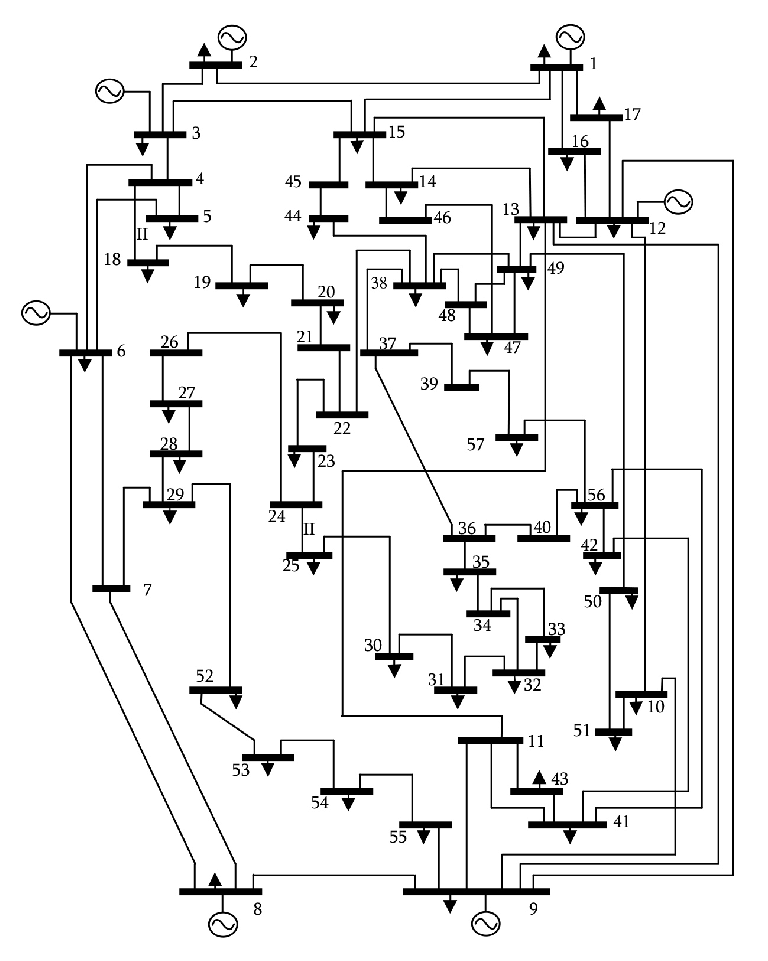
\includegraphics[scale=0.5]{IEEE57BusSystem.png}
\caption{IEEE57 system representation}
\label{circuit-1}
\end{figure}

\subsection{Models}

The generators are modeled as four windings synchronous generators models with a proportional voltage regulator and a proportional speed governor (transformers are included into the machine model; saturations are not represented).

The voltage regulator is as follows:
\begin{figure}[H]
\centering
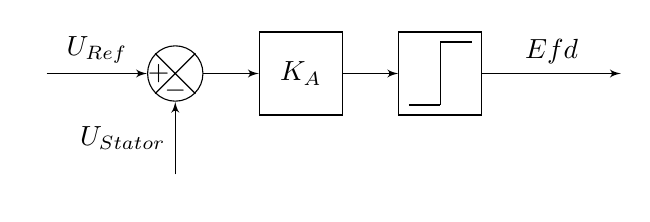
\begin{tikzpicture}
\sbEntree{E}
\sbCompSum[5]{errAVR}{E}{}{-}{+}{}
\sbRelier[$U_{Ref}$]{E}{errAVR}
\sbDecaleNoeudy[4]{errAVR}{Us}
\sbRelier[$U_{Stator}$]{Us}{errAVR}
\sbBloc{Gain}{$K_A$}{errAVR}
\sbRelier{errAVR}{Gain}
\sbBlocL{Limiter}{\tikz {\draw (-0.4,-0.4) -- (0,-0.4);\draw (0,-0.4) -- (0,0.4); \draw (0,0.4) -- (0.4,0.4); }}{Gain}
\sbSortie[5]{S}{Limiter}
\sbRelier[$Efd$]{Limiter}{S}
\end{tikzpicture}
\caption{Voltage regulator}
\end{figure}

The speed governor is as follows - omegaRef being 1 pu in this control scheme -:
\begin{figure}[H]
\centering
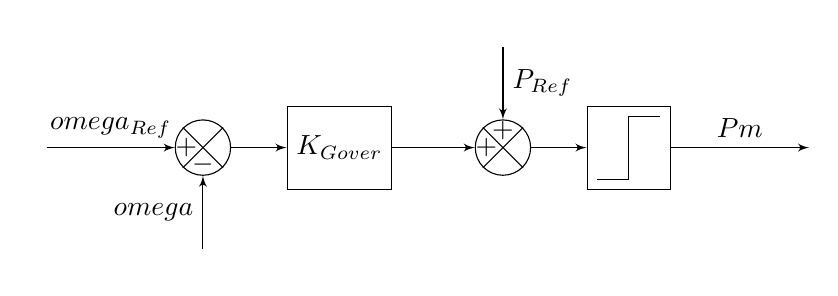
\begin{tikzpicture}
\sbEntree{E}
\sbCompSum[6]{errW}{E}{}{-}{+}{}
\sbRelier[$omega_{Ref}$]{E}{errW}
\sbDecaleNoeudy[4]{errW}{Omega}
\sbRelier[$omega$]{Omega}{errW}
\sbBloc{Gain}{$K_{Gover}$}{errW}
\sbRelier{errW}{Gain}
\sbCompSum{sumP}{Gain}{+}{}{+}{}
\sbRelier{Gain}{sumP}
\sbDecaleNoeudy[-4]{sumP}{PRef}
\sbRelier[$P_{Ref}$]{PRef}{sumP}
\sbBlocL{Limiter}{\tikz {\draw (-0.4,-0.4) -- (0,-0.4);\draw (0,-0.4) -- (0,0.4); \draw (0,0.4) -- (0.4,0.4); }}{sumP}
\sbSortie[5]{S}{Limiter}
\sbRelier[$Pm$]{Limiter}{S}
\end{tikzpicture}
\caption{Speed Governor}
\end{figure}

The loads are modeled as voltage-dependent loads:
\begin{equation*}
\begin{aligned}
& P = P_{0} * (\frac{U}{U_{0}})^\alpha \\
& Q = Q_{0} * (\frac{U}{U_{0}})^\beta
\end{aligned}
\label{Voltage-dependent load model}
\end{equation*}

The system reference frequency is calculated by the OmegaRef model using the different generators speeds.\\

All the models parameters can be viewed into the par file available in the different test case directories.

\subsection{Scenarios}
The simulated scenarios are :
\begin{itemize}
\item a load variation on node 9 [\ref{LoadVariation}];
\item a disconnection of the generator connected to node 12 [\ref{DisconnectGenerator}];
\item a disconnection of the 6-8 line [\ref{DisconnectLine}]
\end{itemize}

\subsection{Solver}
All scenarios are simulated with the variable time step solver IDA using the following parameters:
\begin{itemize}
\item $Order$=2;
\item $Accuracy_{Rel}$=10e-4;
\item $Accuracy_{Abs}$=10e-4;
\end{itemize}

In addition, the line disconnection is also simulated with the simplified solver using in particular the following values:
\begin{itemize}
\item $h_{Max}$=1s;
\item recalculateStep=false;
\end{itemize}

The complete set of parameters used for the solvers are available into the solvers.par file in each test case directory.

\newpage
\section{Results}

\subsection{Load variation}
\label{LoadVariation}

At $t=1s$, the active and reactive power set points for the load on node 9 are doubled. The load value on node 9 is initially multiplied by 2 at $t=1s$ as expected and decreases in the next instants to stabilize at a lower value (due to the voltage-dependent model used). \\

The load increase induces an higher active power demand from the network to the generators and causes a speed decrease. The governor's proportional action limits this speed decrease by increasing the final active power delivered by the machines. Without the regulation action, the final active power delivered by the machines - after the transient behavior - would have been similar to the pre-event active power. \\

Regarding reactive power, it increases after the event to compensate for the load increase. The reactive power increase is stabilized at a value enabling to maintain the stator voltage close to its reference value thanks to the voltage regulator action: this action also enables to limit the voltage decrease on the network.

\begin{figure}[H]
\subfigure[Active load (MW)]
{%
  \begin{tikzpicture}
    \begin{axis}[height = 2in]
        \addplot[color=blue!50]
        table[x=time, y expr= \thisrow{_LOAD____9_EC_load_PPu}*100]
        {../IEEE57_1_StepLoad/reference/outputs/curves/curves.csv};
    \end{axis}
  \end{tikzpicture}
}
\subfigure[Reactive load (Mvar)]
{%
  \begin{tikzpicture}
    \begin{axis}[height = 2in]
        \addplot[color=blue!50]
        table[x=time, y expr=\thisrow{_LOAD____9_EC_load_QPu}*100]
        {../IEEE57_1_StepLoad/reference/outputs/curves/curves.csv};
    \end{axis}
  \end{tikzpicture}
}
\subfigure[Network voltage (kV)]
{%
  \begin{tikzpicture}
    \begin{axis}[height = 2in]
        \addplot[color=blue!50]
        table[x=time, y expr=\thisrow{NETWORK__SALT___9_TN_Upu_value}*69]
        {../IEEE57_1_StepLoad/reference/outputs/curves/curves.csv};
    \end{axis}
  \end{tikzpicture}
}
\caption{Load variation and voltage evolution on node 9}
\end{figure}

\begin{figure}[H]
\subfigure[Active power (MW)]
{%
  \begin{tikzpicture}
    \begin{axis}[height = 1.5in]
        \addplot[color=blue!50]
        table[x=time, y=GEN____9_SM_generator_PGen]
        {../IEEE57_1_StepLoad/reference/outputs/curves/curves.csv};
    \end{axis}
  \end{tikzpicture}
}
\subfigure[Omega (pu)]
{%
  \begin{tikzpicture}
    \begin{axis}[height = 1.5in, yticklabel style={/pgf/number format/.cd,fixed zerofill,precision=3}]
        \addplot[color=blue!50]
        table[x=time, y=GEN____9_SM_generator_omegaPu]
        {../IEEE57_1_StepLoad/reference/outputs/curves/curves.csv};
    \end{axis}
  \end{tikzpicture}
}
\subfigure[Reactive power (Mvar)]
{%
  \begin{tikzpicture}
    \begin{axis}[height = 1.5in]
        \addplot[color=blue!50]
        table[x=time, y=GEN____9_SM_generator_QGen]
        {../IEEE57_1_StepLoad/reference/outputs/curves/curves.csv};
    \end{axis}
  \end{tikzpicture}
}
\subfigure[Stator voltage (kV)]
{%
  \begin{tikzpicture}
    \begin{axis}[height = 1.5in]
        \addplot[color=blue!50]
        table[x=time, y expr=\thisrow{GEN____9_SM_generator_UStatorPu}*20]
        {../IEEE57_1_StepLoad/reference/outputs/curves/curves.csv};
    \end{axis}
  \end{tikzpicture}
}
\caption{Generator 9 response to the load variation}
\end{figure}

\newpage
\subsection{Generator disconnection}
\label{DisconnectGenerator}

At $t=1s$, the generator connected to the node 12 is disconnected. To compensate for this disconnection, the other generators have to increase the active and reactive power delivered to the network in a similar way than for the load increase. It leads to a similar dynamic behavior than for the load increase: the control actions contribute to limit the speed and voltage deviations from the reference values.

\begin{figure}[H]
\subfigure[Active power (MW)]
{%
  \begin{tikzpicture}
    \begin{axis}[height = 1.3in]
        \addplot[color=blue!50]
        table[x=time, y=GEN____1_SM_generator_PGen]
        {../IEEE57_2_DisconnectGroup/reference/outputs/curves/curves.csv};
    \end{axis}
  \end{tikzpicture}
}
\subfigure[Omega (pu)]
{%
  \begin{tikzpicture}
    \begin{axis}[height = 1.3in, yticklabel style={/pgf/number format/.cd,fixed zerofill,precision=3}]
        \addplot[color=blue!50]
        table[x=time, y=GEN____1_SM_generator_omegaPu]
        {../IEEE57_2_DisconnectGroup/reference/outputs/curves/curves.csv};
    \end{axis}
  \end{tikzpicture}
}
\subfigure[Reactive power (Mvar)]
{%
  \begin{tikzpicture}
    \begin{axis}[height = 1.3in]
        \addplot[color=blue!50]
        table[x=time, y=GEN____1_SM_generator_QGen]
        {../IEEE57_2_DisconnectGroup/reference/outputs/curves/curves.csv};
    \end{axis}
  \end{tikzpicture}
}
\subfigure[Stator voltage (kV)]
{%
  \begin{tikzpicture}
    \begin{axis}[height = 1.3in]
        \addplot[color=blue!50]
        table[x=time, y expr=\thisrow{GEN____1_SM_generator_UStatorPu}*20]
        {../IEEE57_2_DisconnectGroup/reference/outputs/curves/curves.csv};
    \end{axis}
  \end{tikzpicture}
}
\caption{Generator 1 response to the disconnection}
\end{figure}

\newpage
\subsection{Line Opening}
\label{DisconnectLine}

At $t=1s$, we open the direct line between the nodes 6 and 8.We observe that the system is oscillating after the event but stabilizes after a few seconds. The active power is restored to its pre-event value and the generator speeds remains quasi-constant but the reactive power is changed in response to the stator voltage change (action of the voltage regulation).

\begin{figure}[H]
\subfigure[Active power (MW)]
{%
  \begin{tikzpicture}
    \begin{axis}[height = 1.3in]
        \addplot[color=blue!50]
        table[x=time, y=GEN____8_SM_generator_PGen]
        {../IEEE57_3_DisconnectLine/reference/outputs/curves/curves.csv};
    \end{axis}
  \end{tikzpicture}
}
\subfigure[Omega (pu)]
{%
  \begin{tikzpicture}
    \begin{axis}[height = 1.3in, yticklabel style={/pgf/number format/.cd,fixed zerofill,precision=3}]
        \addplot[color=blue!50]
        table[x=time, y=GEN____8_SM_generator_omegaPu]
        {../IEEE57_3_DisconnectLine/reference/outputs/curves/curves.csv};
    \end{axis}
  \end{tikzpicture}
}
\subfigure[Reactive power (Mvar)]
{%
  \begin{tikzpicture}
    \begin{axis}[height = 1.3in]
        \addplot[color=blue!50]
        table[x=time, y=GEN____8_SM_generator_QGen]
        {../IEEE57_3_DisconnectLine/reference/outputs/curves/curves.csv};
    \end{axis}
  \end{tikzpicture}
}
\subfigure[Stator voltage (kV)]
{%
  \begin{tikzpicture}
    \begin{axis}[height = 1.3in]
        \addplot[color=blue!50]
        table[x=time, y expr=\thisrow{GEN____8_SM_generator_UStatorPu}*24]
        {../IEEE57_3_DisconnectLine/reference/outputs/curves/curves.csv};
    \end{axis}
  \end{tikzpicture}
}
\caption{Generator 8 response to the disconnection}
\end{figure}

When the simulation is done with the simplified solver, it naturally filters the fast oscillations (fix time-step equal to one second) but is able to correctly catch the long-term behavior and the new equilibrium point.

\begin{figure}[H]
\subfigure[Active power (MW)]
{%
  \begin{tikzpicture}
    \begin{axis}[height = 1.3in]
        \addplot[color=blue!50]
        table[x=time, y=GEN____8_SM_generator_PGen]
        {../IEEE57_3_DisconnectLine/reference/outputsSIM/curves/curves.csv};
    \end{axis}
  \end{tikzpicture}
}
\subfigure[Omega (pu)]
{%
  \begin{tikzpicture}
    \begin{axis}[height = 1.3in, yticklabel style={/pgf/number format/.cd,fixed zerofill,precision=3}]
        \addplot[color=blue!50]
        table[x=time, y=GEN____8_SM_generator_omegaPu]
        {../IEEE57_3_DisconnectLine/reference/outputsSIM/curves/curves.csv};
    \end{axis}
  \end{tikzpicture}
}
\subfigure[Reactive power (Mvar)]
{%
  \begin{tikzpicture}
    \begin{axis}[height = 1.3in]
        \addplot[color=blue!50]
        table[x=time, y=GEN____8_SM_generator_QGen]
        {../IEEE57_3_DisconnectLine/reference/outputsSIM/curves/curves.csv};
    \end{axis}
  \end{tikzpicture}
}
\subfigure[Stator voltage (kV)]
{%
  \begin{tikzpicture}
    \begin{axis}[height = 1.3in]
        \addplot[color=blue!50]
        table[x=time, y expr=\thisrow{GEN____8_SM_generator_UStatorPu}*24]
        {../IEEE57_3_DisconnectLine/reference/outputsSIM/curves/curves.csv};
    \end{axis}
  \end{tikzpicture}
}
\caption{Generator 8 response to the disconnection with the simplified solver}
\end{figure}

This is also visible when superposing the active power going onto the lines 6-7 and 7-8 (that were in parallel with the line 6-8 being disconnected) with the two solvers.

\begin{figure}[H]
\subfigure[Active power on line 6-7]
{%
  \begin{tikzpicture}
    \begin{axis}[height = 2.5in]
        \addplot[color=blue!50]
        table[x=time, y expr=\thisrow{NETWORK__BEAV___6-BUS____7-1_AC_P2_value}*100]
        {../IEEE57_3_DisconnectLine/reference/outputs/curves/curves.csv};
        \addplot[color=red!50]
        table[x=time, y expr=\thisrow{NETWORK__BEAV___6-BUS____7-1_AC_P2_value}*100]
        {../IEEE57_3_DisconnectLine/reference/outputsSIM/curves/curves.csv};
        \legend{IDA Solver, Simplified Solver}
    \end{axis}
  \end{tikzpicture}
}
\subfigure[Active power on line 7-8]
{%
  \begin{tikzpicture}
    \begin{axis}[height = 2.5in]
        \addplot[color=blue!50]
        table[x=time, y expr=\thisrow{NETWORK__BUS____7-CLIN___8-1_AC_P1_value}*100]
        {../IEEE57_3_DisconnectLine/reference/outputs/curves/curves.csv};
        \addplot[color=red!50]
        table[x=time, y expr=\thisrow{NETWORK__BUS____7-CLIN___8-1_AC_P1_value}*100]
        {../IEEE57_3_DisconnectLine/reference/outputsSIM/curves/curves.csv};
        \legend{IDA Solver, Simplified Solver}
    \end{axis}
  \end{tikzpicture}
}
\caption{Active power on remaining lines with IDA and simplified solvers}
\end{figure}

\end{document}
